\documentclass{letter}
\usepackage{wallpaper}
\usepackage{geometry}
\usepackage{xcolor}
\usepackage[T1]{fontenc}
\usepackage[scaled]{helvet}
\usepackage{fontawesome5}
\usepackage[hidelinks]{hyperref}
\usepackage[none]{hyphenat}
\usepackage{graphicx}
\usepackage{tikz}
\usetikzlibrary{calc}

\renewcommand{\familydefault}{\sfdefault}

\geometry{
  paperwidth=\dimexpr\textwidth+\marginparsep+\marginparwidth\relax,
  paperheight=\dimexpr\textheight+\footskip\relax,
  left=20pt,
  right=20pt,
  top=0pt,
  bottom=0pt,
  nohead,
  nofoot,
  nomarginpar
}

\ThisCenterWallPaper{1.5}{cvbg.png}

% Custom command for dividers
\newcommand{\divider}{\rule{\linewidth}{0.9pt}}

% ============================================================
% ======================== Left Side =========================
% ============================================================


\begin{document}
\small
\begin{minipage}[t]{0.40\textwidth}
\setlength{\baselineskip}{1.5\baselineskip}
\color{white}
\vspace{5mm}

% ========================== Photo ============================

\begin{tikzpicture}
    \clip (0,0) circle (2cm);
    \node[anchor=center] at (0,0) {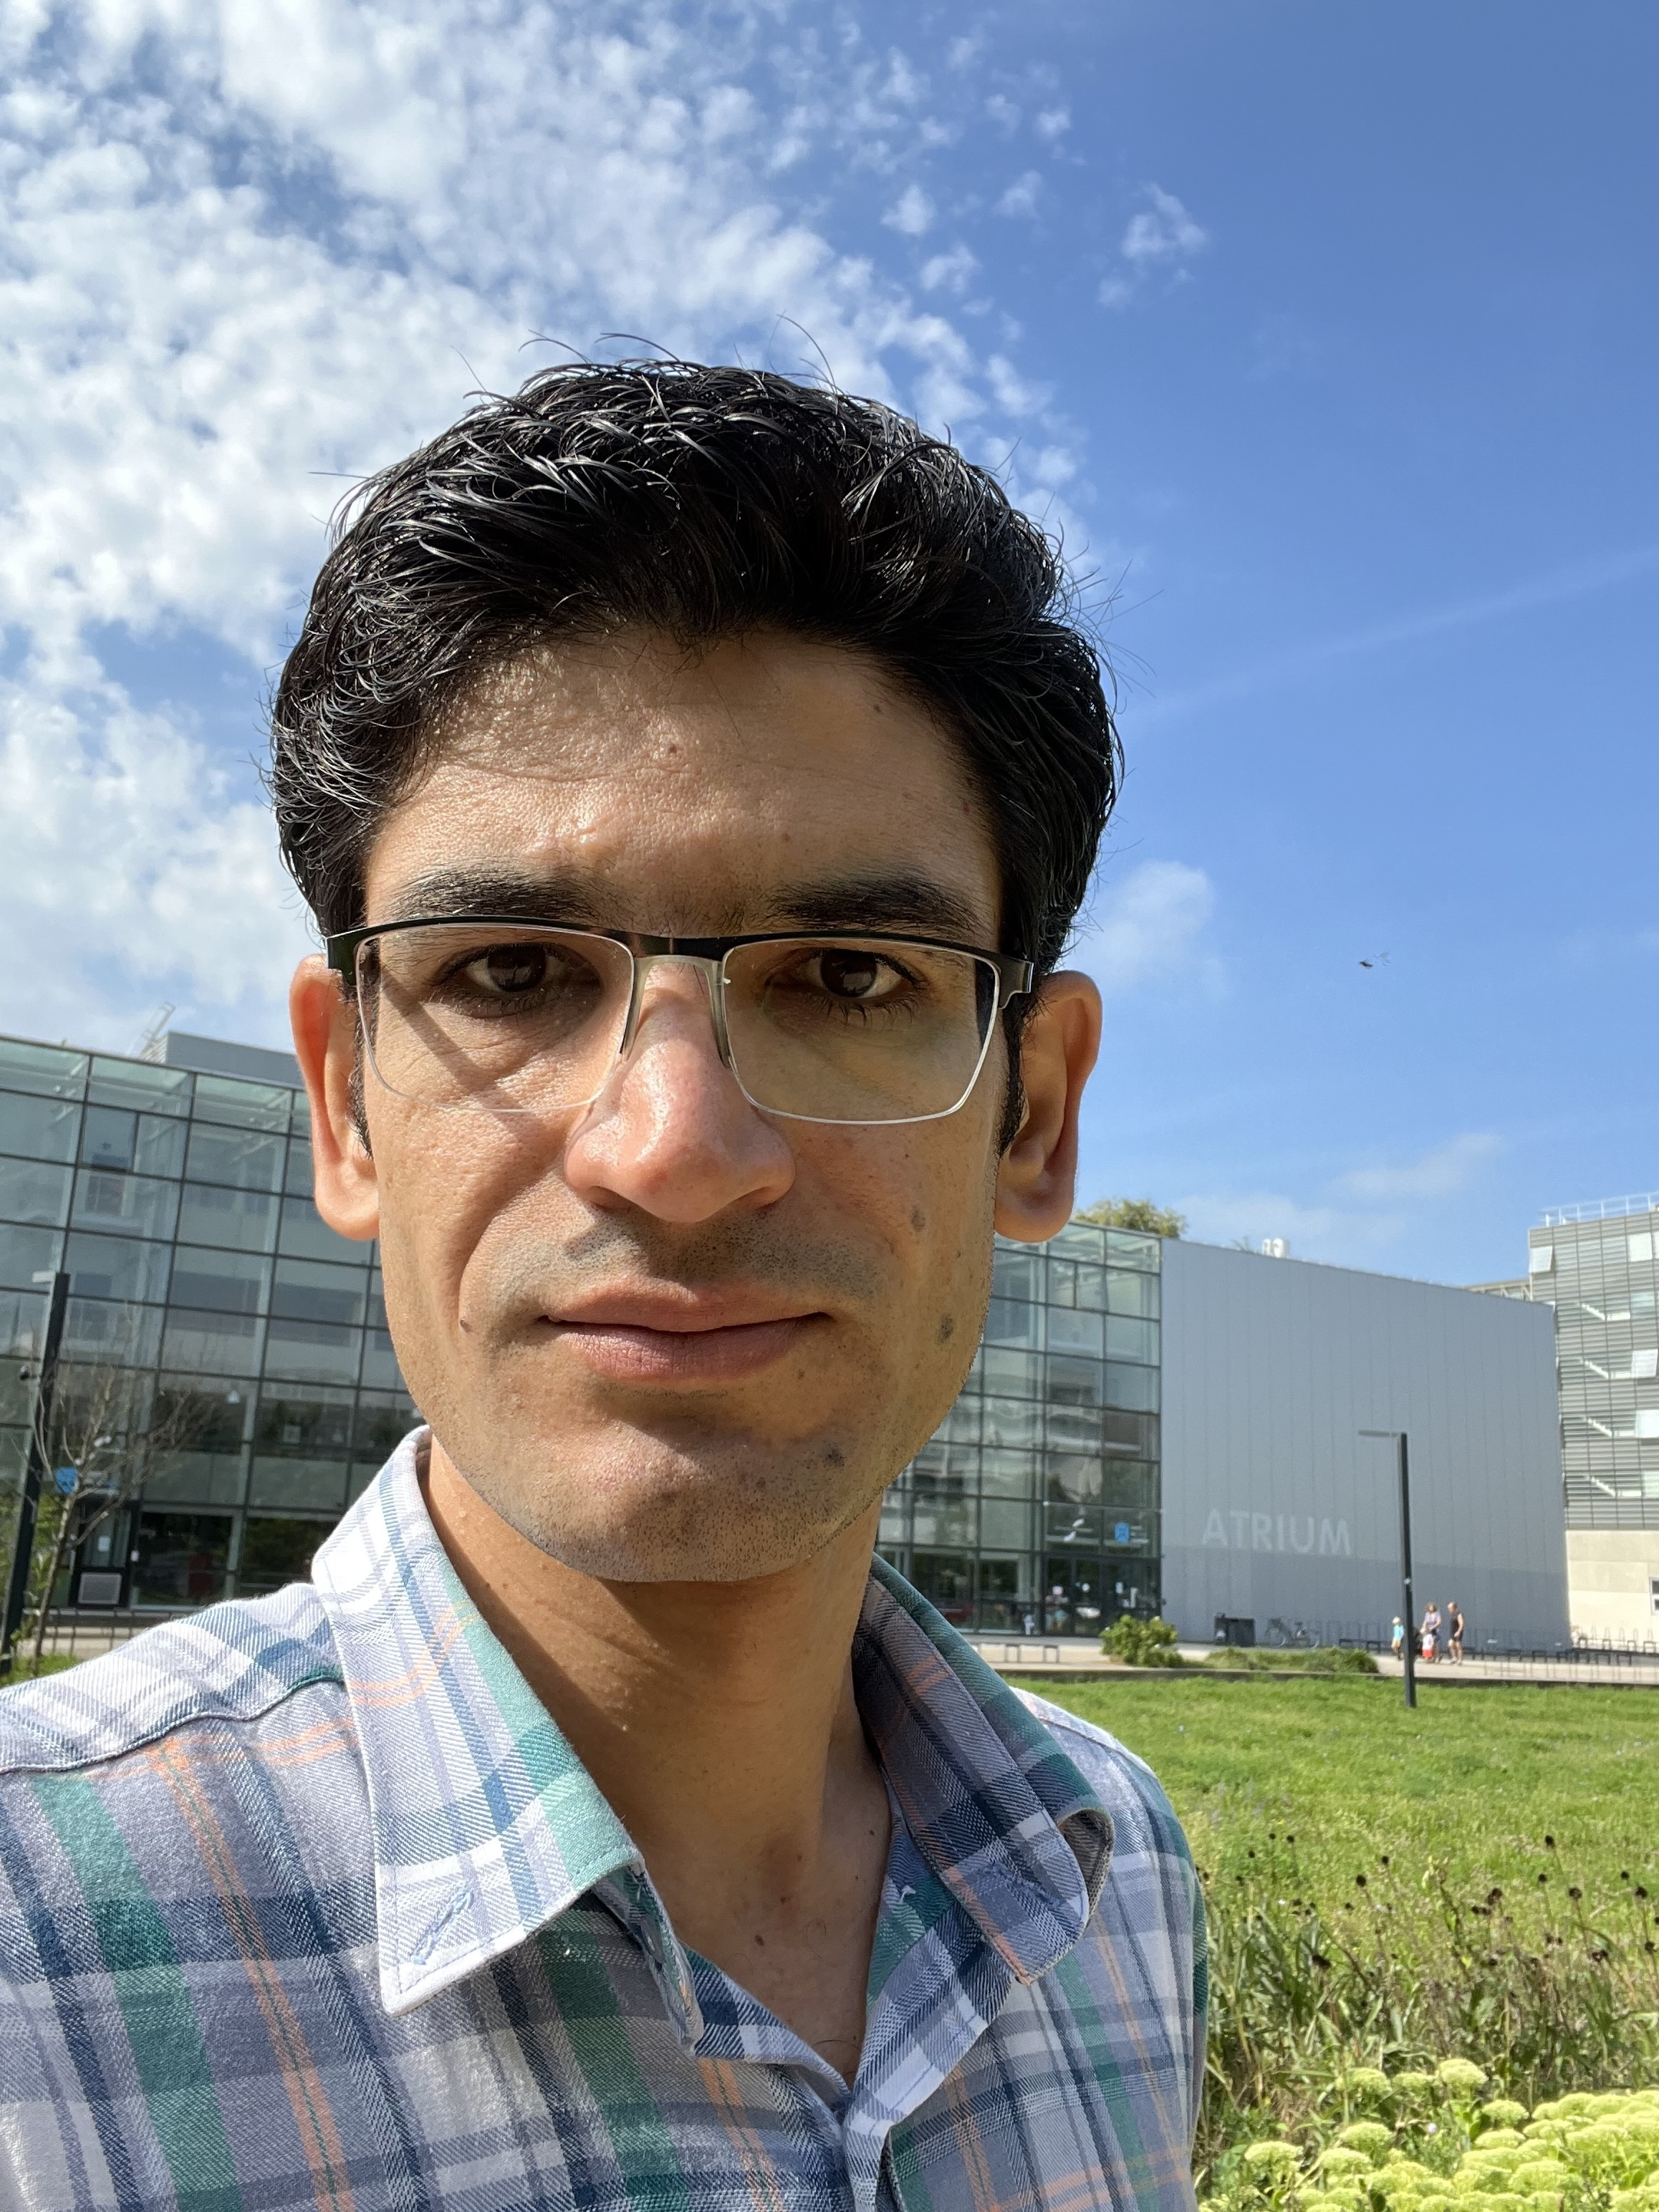
\includegraphics[width=4cm]{profile.jpg}};
\end{tikzpicture}

\vspace{5mm}

\divider

% ========================= Contact ===========================

\faPhone \quad 06 52 22 49 24

\faEnvelope \quad jafarizadeh89@gmail.com

\faGithub \quad \href{https://github.com/jafarizadeh}{jafarizadeh}

\faLinkedin \quad \href{https://www.linkedin.com/in/jafarizadeh/}{linkedin.com/in/jafarizadeh/}


\divider

% =================== programming language ===================

{\large \textbf{programming language}}

\faCircleNotch \quad Python

\faCircleNotch \quad C

\faCircleNotch \quad Swift

\faCircleNotch \quad HTML / CSS

\faCircleNotch \quad JavaScript

\faCircleNotch \quad SQL

\divider

% ====================== CAD Software ========================

{\large \textbf{CAD Software}}

\faCircleNotch \quad AutoCAD

\faCircleNotch \quad CATIA

\divider

% ========================== Network ==========================


{\large \textbf{Network}}

\faNetworkWired \quad CCNA

\faNetworkWired \quad CCNP (ENATSI)

\end{minipage}
\hfill
\begin{minipage}[t]{0.60\textwidth}

% ============================================================
% ======================= Right Side =========================
% ============================================================

\setlength{\baselineskip}{1.5\baselineskip}
\vspace{0.7cm}

{\huge Mehdi JAFARIZADEH}

\vspace{1cm}

% ========================= Education =========================

{\large \textbf{Education}}
\divider

{ \textbf{Accounting (Bachelor +2)}}

{\footnotesize September 2007-December 2010}
\begin{itemize}
    \footnotesize \item \textit{Azad University of Kerman, Kerman}
\end{itemize}

\vspace{3mm}

{ \textbf{Energy Engineering (Bachelor +4)}}

{\footnotesize September 2014-December 2018}
\begin{itemize}
    \footnotesize \item \textit{Technological University of Quchan, Mashhad}
\end{itemize}

\vspace{3mm}

{\textbf{Computer Science}}

{\footnotesize September 2021-Present}
\begin{itemize}
    \footnotesize \item \textit{University of Strasbourg, Strasbourg}
\end{itemize}

\vspace{0.8cm}

% ================= Professional Experience ===================

{\large \textbf{Professional Experience}}
\divider

{ \textbf{Teaching Assistant}}

{ \footnotesize September 2014-December 2017}
\begin{itemize}
    \footnotesize \item \textit{Technological University of Quchan, Mashhad}
\end{itemize}

\vspace{3mm}

{\textbf{Director of the Energy Engineering Association}}

{\footnotesize September 2015-December 2017}
\begin{itemize}
   \footnotesize \item \textit{Technological University of Quchan, Mashhad}
\end{itemize}



\vspace{0.8cm}

% ================== Academic Contributions ===================

{\large \textbf{Academic Contributions}}
\divider
\vspace{4mm}
\begin{itemize}
    \footnotesize \item {\textbf{Co-author}, \textit{Energy Audit Guide for the students of the University of Quchan, with Dr. Majid Mahdavian, Published in 2019}}


\end{itemize}

\vspace{3mm}

\end{minipage}

% ========================== QR Code and Date ==========================

\begin{tikzpicture}[remember picture,overlay]
    % QR Code and description
    \node[anchor=south east,inner sep=0pt] at ($(current page.south east)-(1cm,-1cm)$) {
        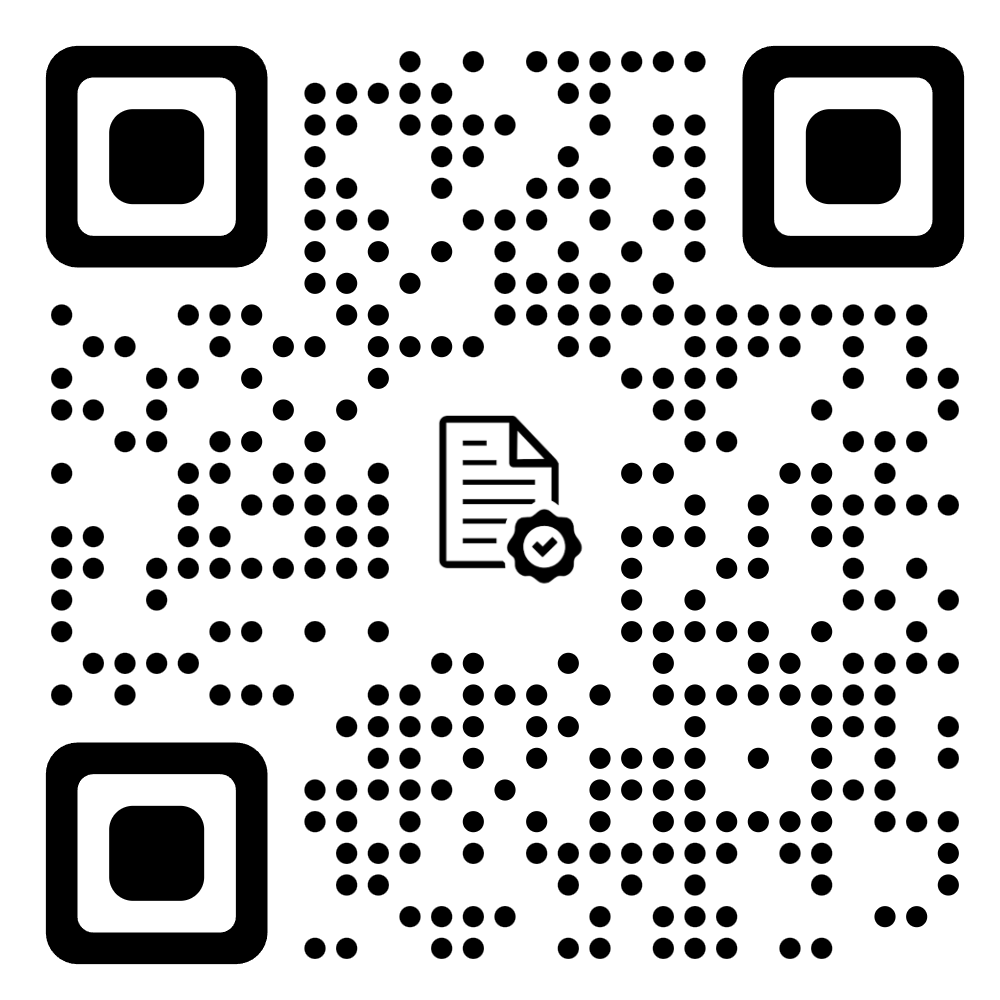
\includegraphics[width=2cm]{Documentation_EN.png}
    };
    
    \node[anchor=south east,inner sep=0pt] at ($(current page.south east)-(3.5cm,-1.2cm)$) {
        \begin{minipage}[t]{2.7cm} 
            \tiny \href{https://drive.google.com/file/d/1SwrSxWrC8iVVY-hpDYJElf16-4BYZWbR/view?usp=drive_link}{Please click here or scan the QR codes to access a detailed file of my academic and professional contributions.}
        \end{minipage}
    };
    
    % Date of last update
    \node[anchor=south west,inner sep=0pt] at ($(current page.south west)+(1cm,1cm)$) {
        \begin{minipage}[t]{4cm}
            \tiny \textcolor{white}{Last updated: \today}
        \end{minipage}
    };
\end{tikzpicture}

\end{document}
